本研究で製作したロボットを用いて,歩行実験を行う.
この実験の目的として,倒立振子モデルの特徴である,

\begin{enumerate}
 \item 支持脚長の変化
 \item 重心軌道
\end{enumerate}

について,歩行中の挙動の解析を目的とする.



\subsection{歩行動作生成}
本研究では,単純な制御によって動くロボットの実現を目的としている.
これを達成するため,ロボットの動作生成手法として,フィードフォワード制御を用いる.
実際には,歩行動作を単純な周期運動であると見なし,あらかじめモータの角度遷移や各筋への給排気パターンを繰り返すという手法を用いる.
ただし,ロボットの初期状態を一定にするため,直立状態を初期状態とし,1歩目のモータおよび空気圧人工筋のパラメータは別の値を用意することとする.

実際に,実験で使用した歩行パラメータパターンをFig.\ref{parameter}に示す.
全ての筋において,給排気の切り替えのタイミングは100msecごとで統一している.
モータの角度は,100msecごとに目標角度値を設定しており,20msecごとに前後の目標角度値の内分点に追従するように動作させている.
また,各筋の給排気パターン及びモータの目標角度値は,実験者が,前述の空気圧人工筋内の圧力値と関節角度の対応を参考に,試行錯誤的に決定したパラメータである.

図の縦の点線は,パラメータの切り替えのタイミングを示しており,1周期を800[msec]に設定した.
横の点線は,1目盛が10[deg]の間隔をとっている.
股関節にあるモータの目標角度について,ピッチ軸は,地面と垂直な状態を0[deg]とし,屈曲を正,伸展を負の角度として設定している.
また,ロール軸も同様に,地面と垂直な状態を0[deg]とし,内転を正,外転を負の角度として設定している.

実際に,Fig.\ref{parameter}の歩行パラメータパターンを用いて,最大4歩の歩行に成功した.
以下に,歩行パラメータの説明を行う.

\begin{description}
\item[支持脚期] \mbox{}
 \begin{enumerate}
  \item 距腿関節と股関節の動作によって,ロボットの重心を大きく前方に倒す.
  \item 重心を前に倒した状態を維持する.
  \item ヒラメ筋を収縮させることで,スムーズな重心移動を実行する.
  \item ヒラメ筋を再び伸長させ,重心移動を慣性によって実行する.
 \end{enumerate}
\item[遊脚期] \mbox{}
 \begin{enumerate}
  \item 距腿関節と股関節の動作によって,ロボットの重心を前方に倒しつつ,次の遊脚を屈曲させる準備をする.
  \item 後ろの支持脚で蹴り出しを行い,そのまま遊脚期に入る.
  \item 遊脚が地面につかないように脚の関節を調節し,脚を前方に大きく振り出す.
  \item 遊脚が支持脚に移行するための準備として,膝関節を伸展状態にさせながら,足部の着く位置を調整する.
 \end{enumerate}
\end{description}
	    
\begin{figure}[htbp]
 \centering
 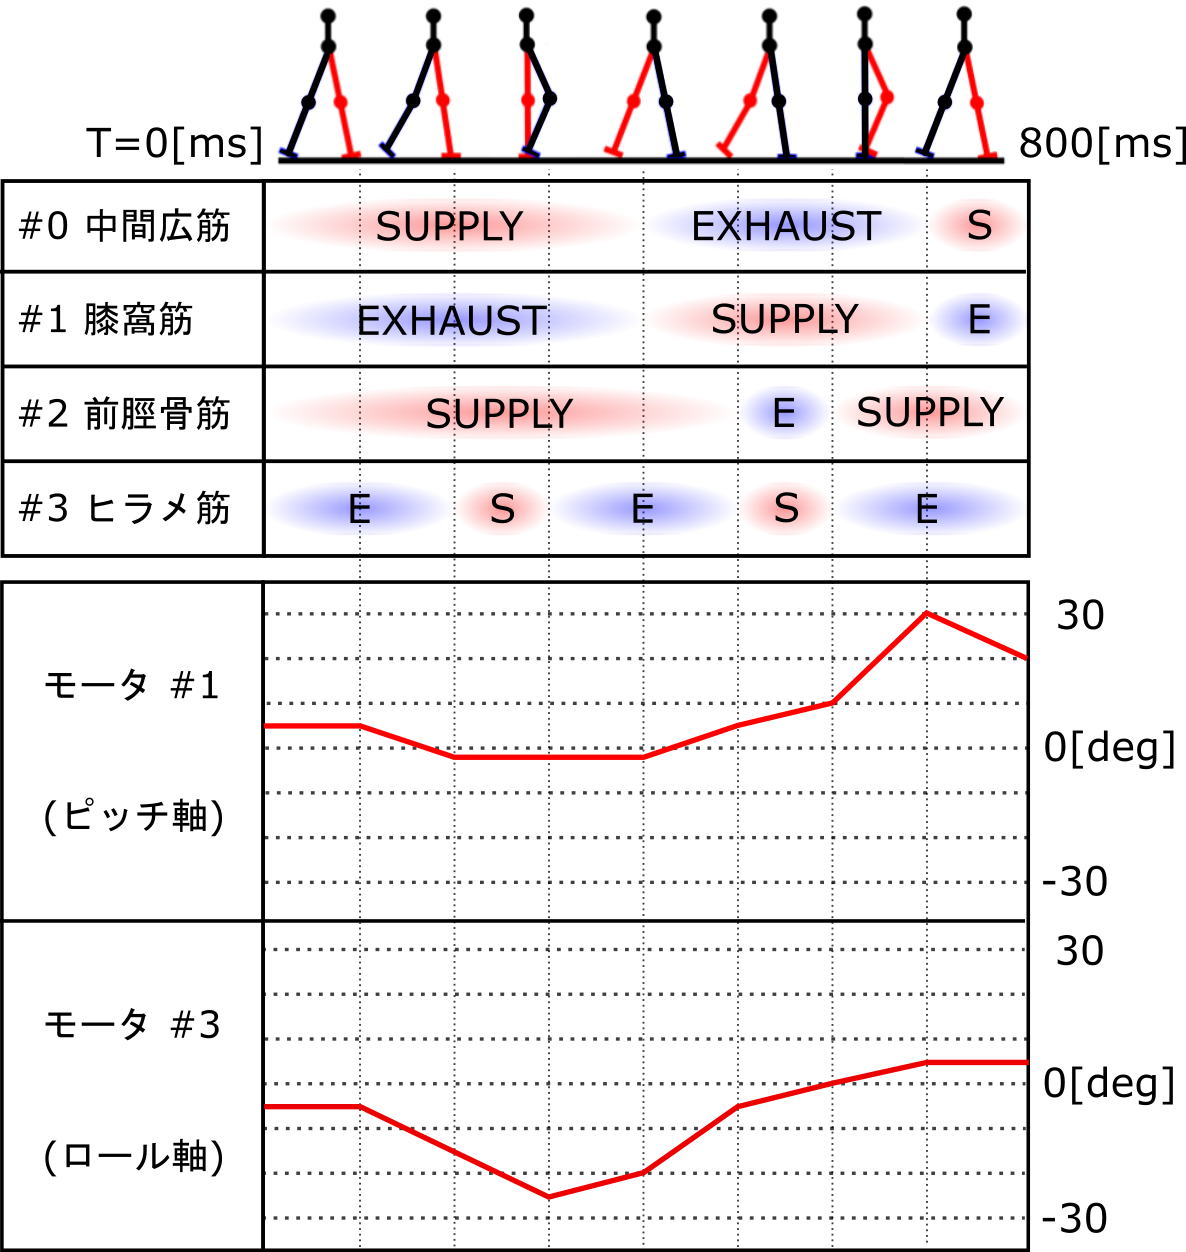
\includegraphics[clip,width=12.0cm]{./fig/parameter_pattern.png}
    \caption{歩行パラメータパターン一覧.図上部の赤く表示された方の脚が,支持脚期から始まる1周期分のパラメータパターンを示している.また,筋のパラメータに書かれているSとEは,それぞれSUPLY,EXHAUSTのことであり,給気と排気を表す.\label{parameter}}
\end{figure}



\subsection{実験環境}
このパラメータを用いて,地面との摩擦を大きくするためにフェルトの布上で歩行実験を行う(Fig.\ref{}).
実験中の試行において,ロボットが最大歩数歩いた実験について,ロボットの関節角度(主に膝関節)の推移と重心移動を計測する.

\subsection{実験結果及び考察}
歩行中のロボットの連続写真をFig.\ref{photoseries}に示す.
本章の始めに述べた,倒立振子モデルがもつ特徴を満たしているかを調べるために,支持脚期における脚の関節角度の推移(Fig.\ref{motioncapture}),及び歩行中の重心位置の推移(Fig.\ref{motioncapture})を,モーションキャプチャを用いて計測した.
また,前者の関節角度の推移については,モーションキャプチャ使用時のマーカ位置によって簡単に確認することができるため,連続写真から分析を行うこととする.

(結果・考察)

\begin{figure}[htbp]
 \centering
 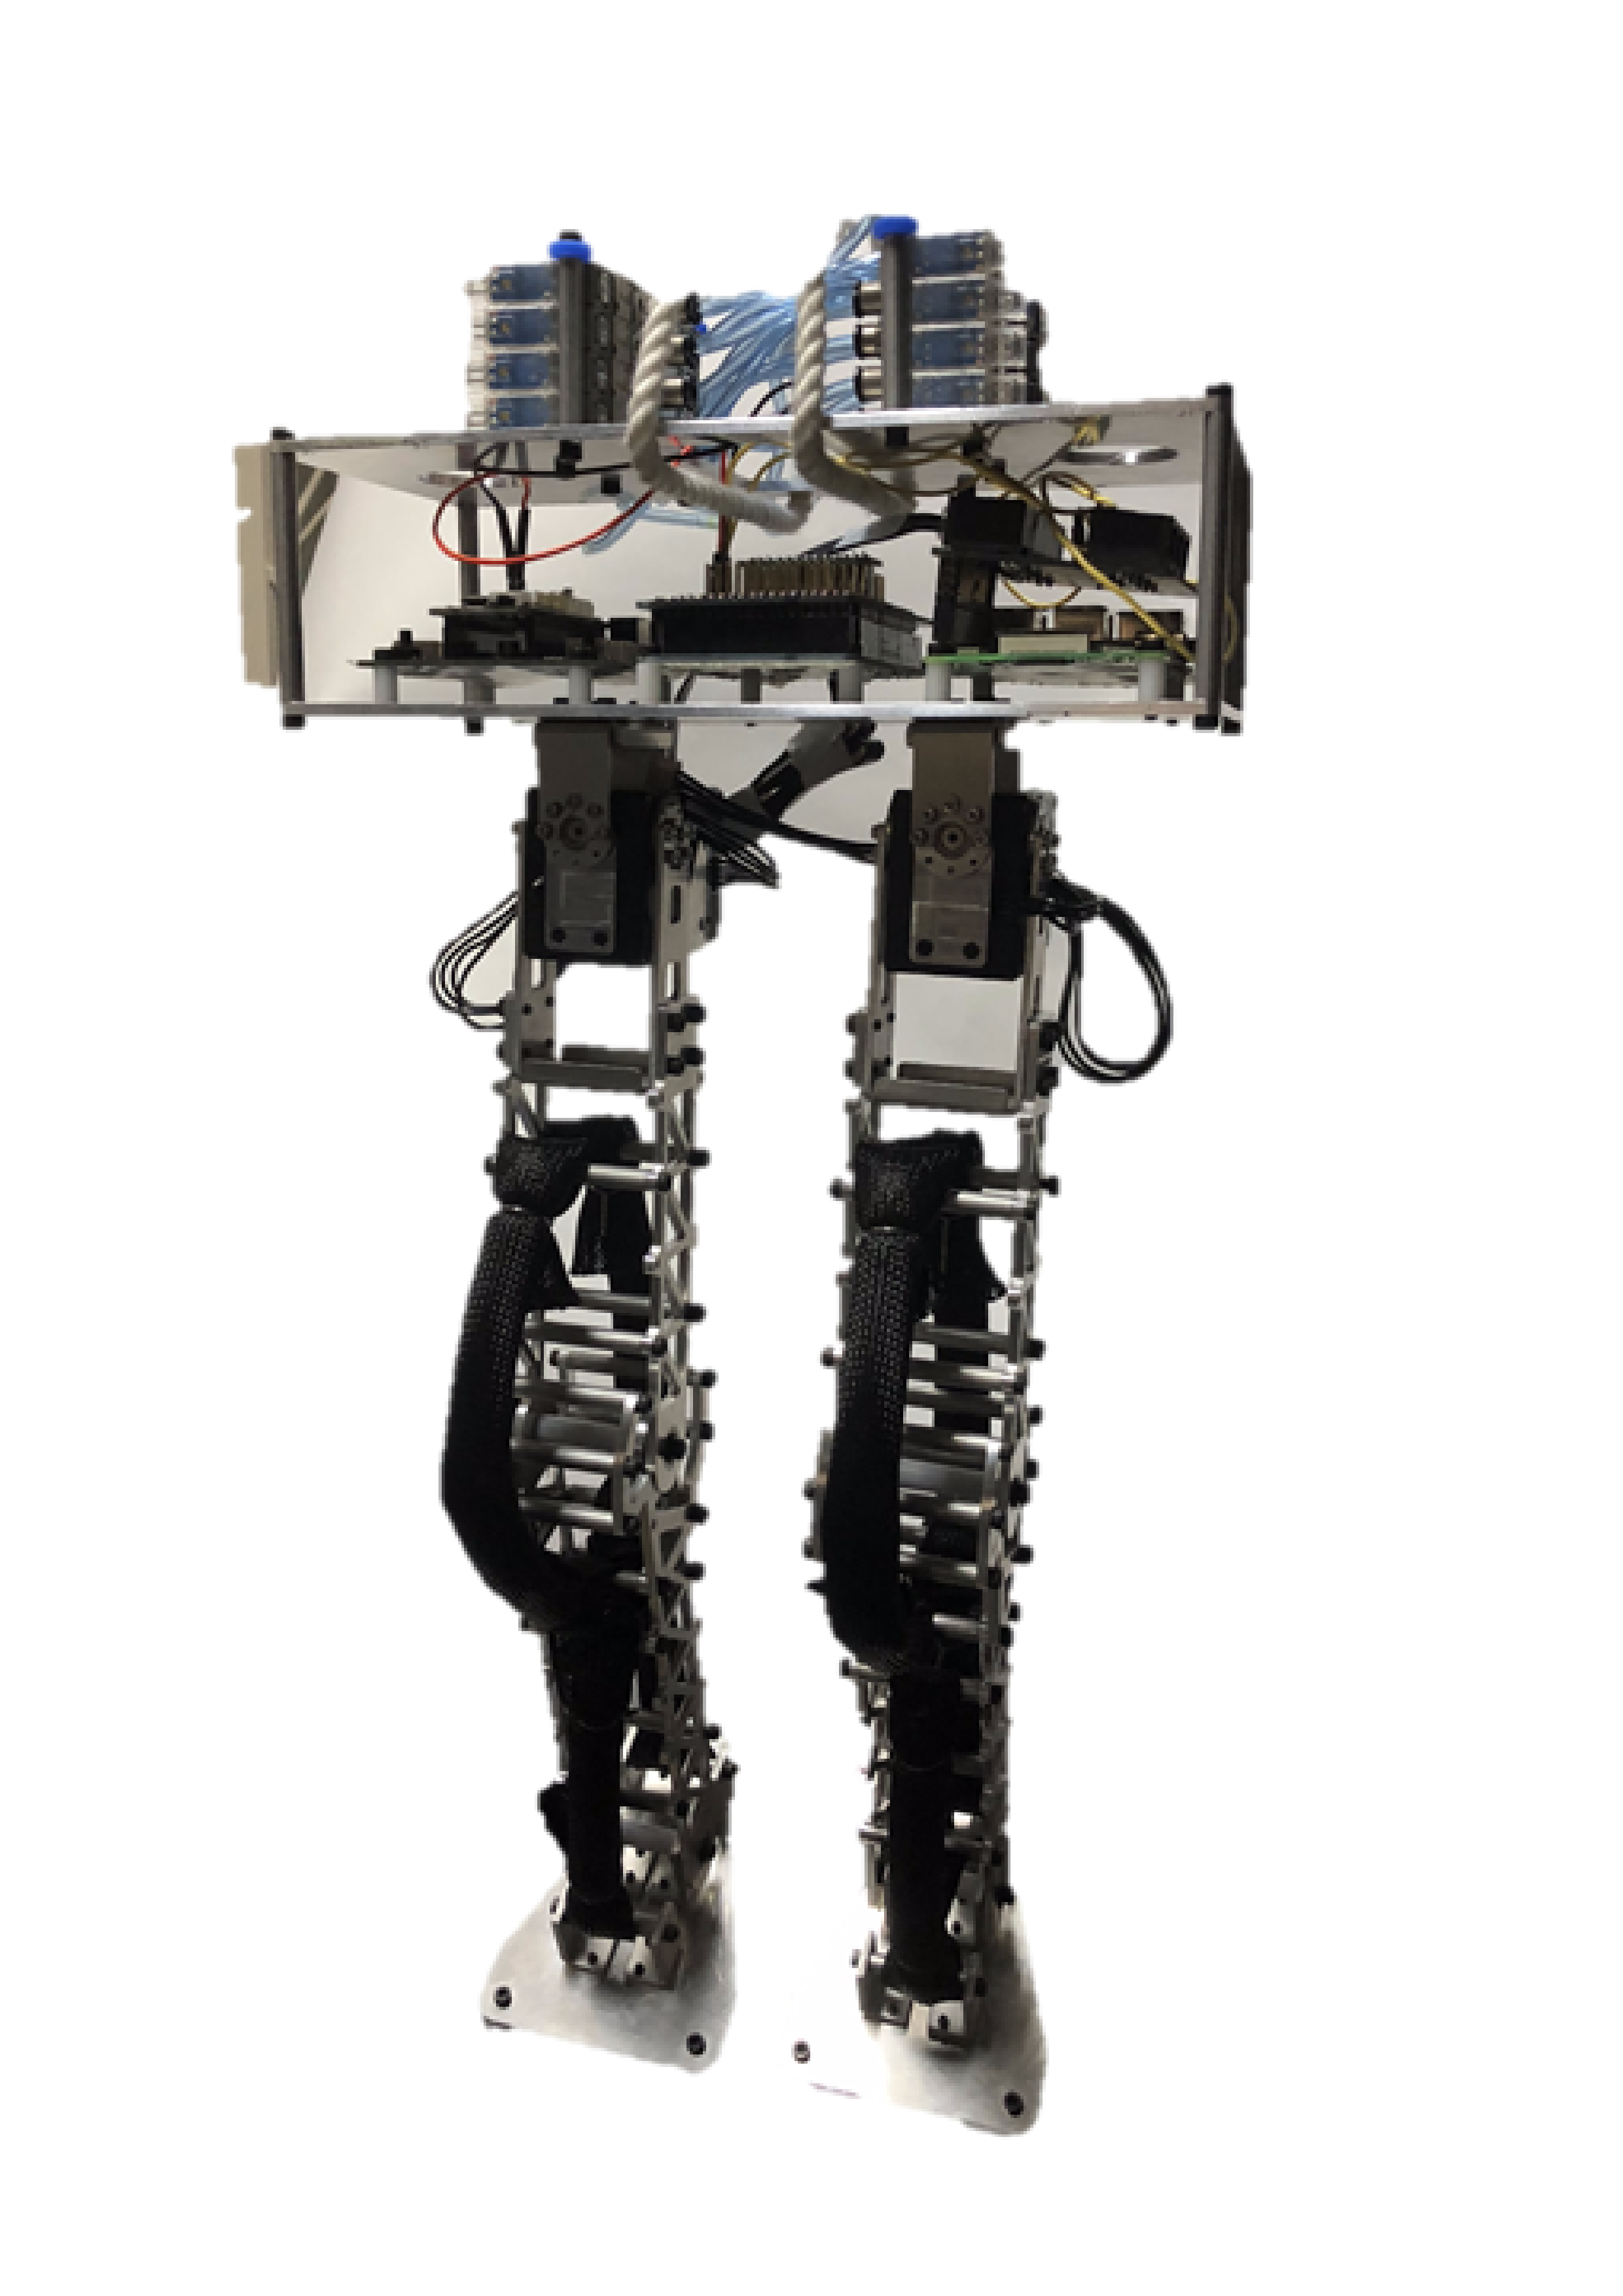
\includegraphics[clip,width=5.0cm]{./fig/robot.png} % 仮
    \caption{歩行中の連続写真.\label{photoseries}}
\end{figure}

\begin{figure}[htbp]
 \centering
 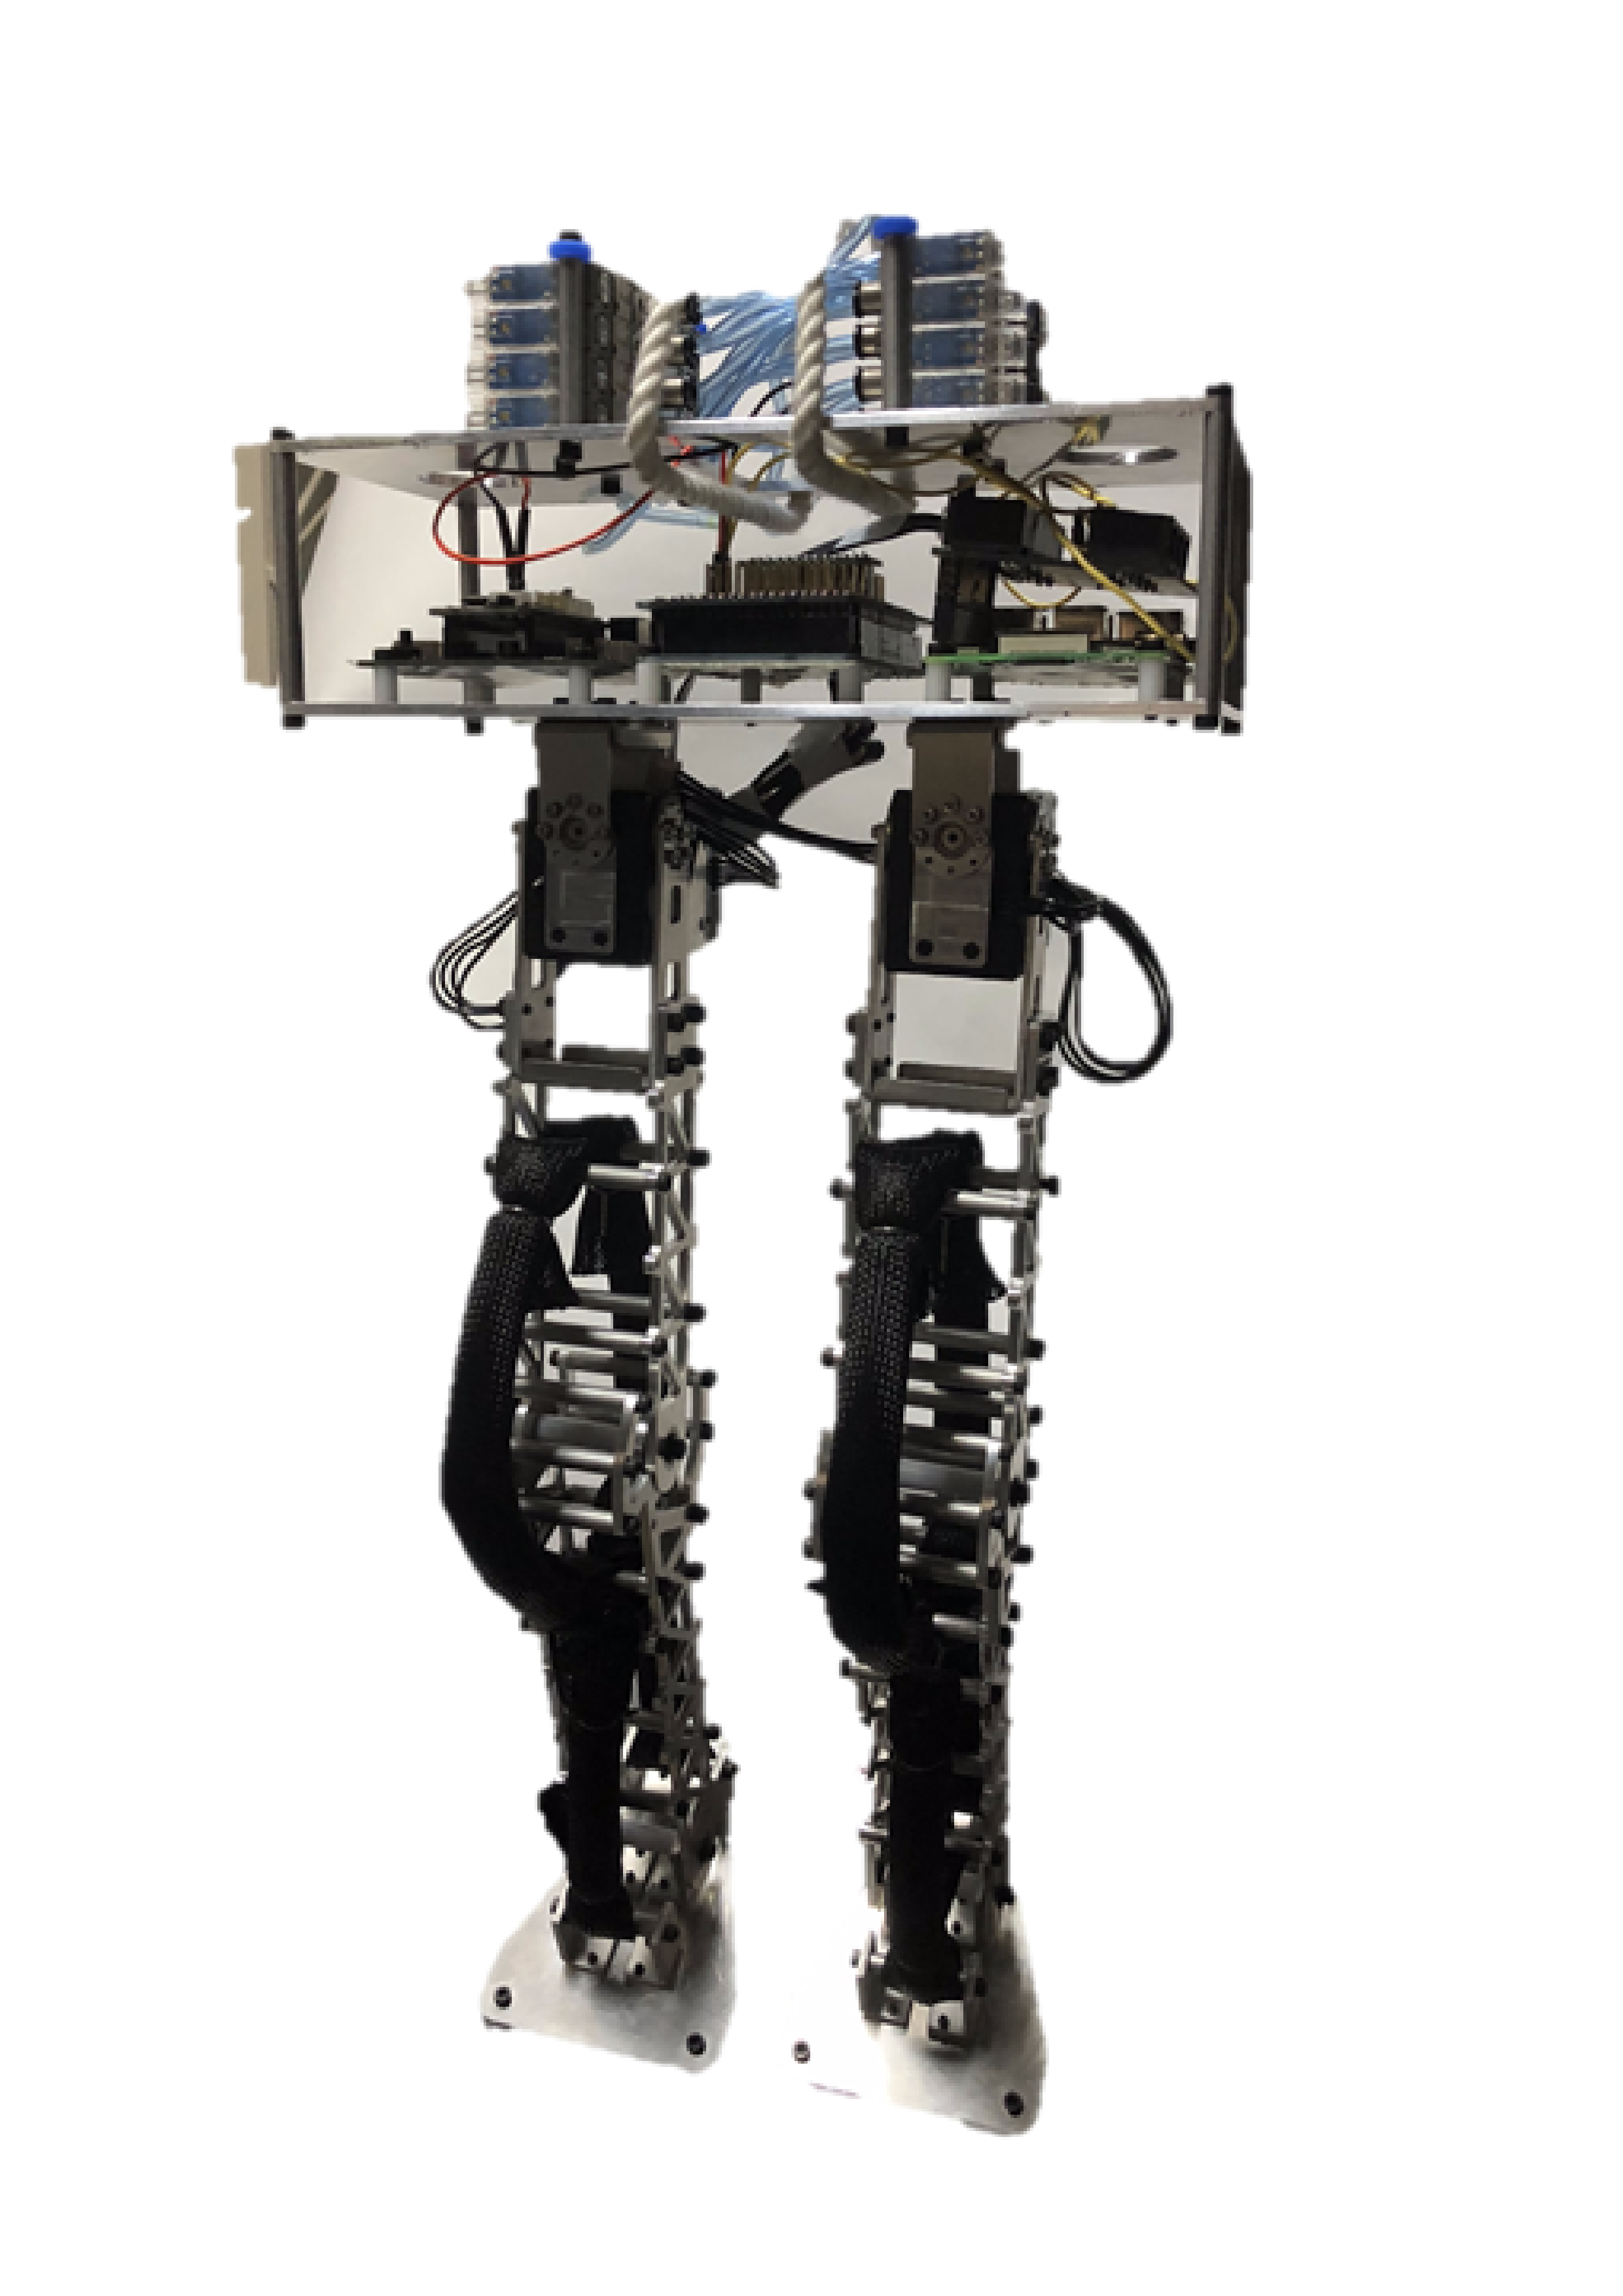
\includegraphics[clip,width=5.0cm]{./fig/robot.png} % 仮
    \caption{モーションキャプチャによる歩行中のロボットのスティック線図.\label{motioncapture}}
\end{figure}

\subsection{走行実験}
本研究では,矢状面方向への速度変化で歩行と走行といった歩容が変化するモデルを提案し,その機構の実装を目標とした.
このため,本ロボットにおいて走行実験も行ったが,走行の一要素である跳躍に必要な力を生み出すことができなかったため,走行を達成することはできなかった.
今回製作したロボットは全長が短く,それに応じて空気圧人工筋の長さも短くする必要があった.
しかし,空気圧人工筋の長さが短いと,収縮長も短くなるため,距腿関節による十分な蹴り出しが行えなかったことが原因であると考えられる.
これを改善するための方法として,距腿関節の底屈に作用する二関節筋である腓腹筋を実装するなどの手法によって,距腿関節の可動域をより大きくすることで改善されるのではないかと考えている.